\documentclass{article}
\usepackage[a4paper,landscape,margin=1.5cm]{geometry}
\usepackage{pgfplots}
\pgfplotsset{compat=1.18}
\pagestyle{empty}
\begin{document}
\section*{\texttt{cnot-S2-by-grouping.tex}}
Suzuki $S_2$: cnot count by grouping (unmerged, measured $r$)\par\medskip
% Generated by plsimcount.pfgrouping -- do not edit; regenerate instead.
% Suzuki S2, cnot, unmerged, cz, seed 1, t = n, measured r
% git_commit=8c69e76829985cb586945dc9e8ed58101f318fe1 git_dirty=False
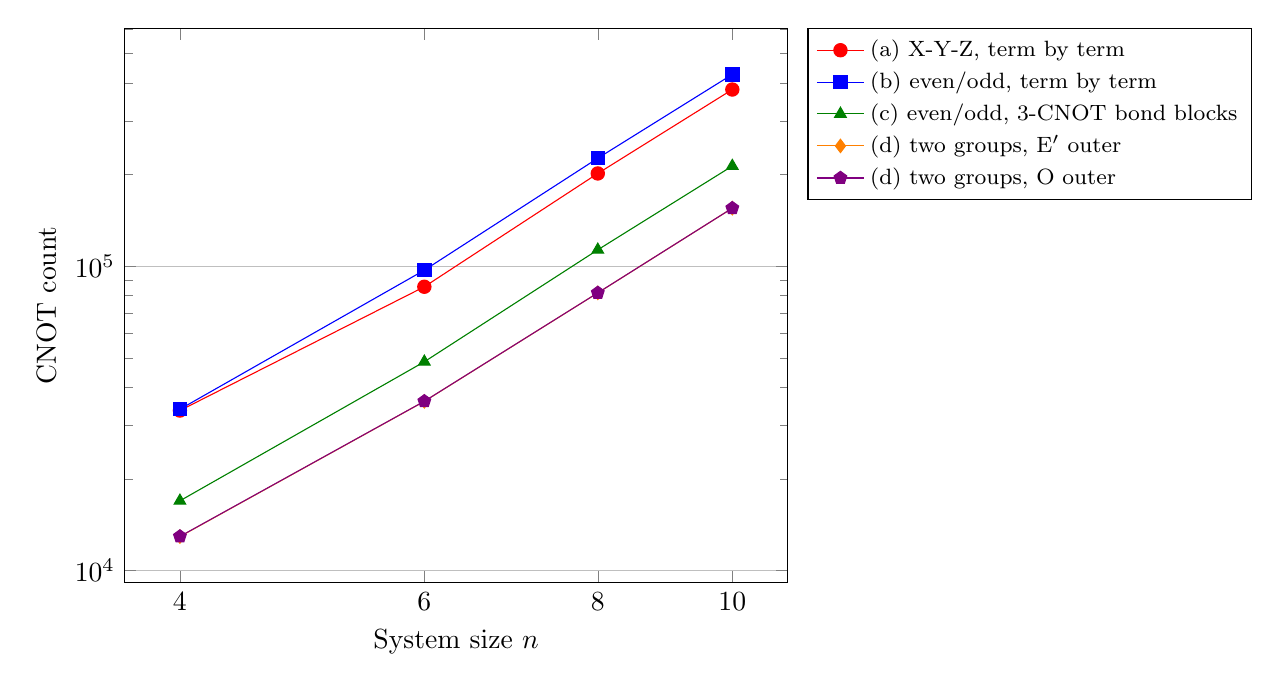
\begin{tikzpicture}
  \begin{loglogaxis}[
    width=10cm,
    xlabel={System size $n$},
    ylabel={CNOT count},
    xtick={4,6,8,10},
    xticklabels={4,6,8,10},
    ymajorgrids=true,
    legend pos=outer north east,
    legend cell align=left,
    legend style={font=\footnotesize},
  ]
    \addplot[red, mark=*, mark size=2.4pt, mark options={solid, fill=red}] coordinates {
      (4,33552)
      (6,85608)
      (8,201792)
      (10,380880)
    };
    \addlegendentry{(a) X-Y-Z, term by term}
    \addplot[blue, mark=square*, mark size=2.4pt, mark options={solid, fill=blue}] coordinates {
      (4,33888)
      (6,97056)
      (8,226464)
      (10,426960)
    };
    \addlegendentry{(b) even/odd, term by term}
    \addplot[green!50!black, mark=triangle*, mark size=2.4pt, mark options={solid, fill=green!50!black}] coordinates {
      (4,16944)
      (6,48528)
      (8,113232)
      (10,213480)
    };
    \addlegendentry{(c) even/odd, 3-CNOT bond blocks}
    \addplot[orange, mark=diamond*, mark size=2.4pt, mark options={solid, fill=orange}] coordinates {
      (4,12924)
      (6,35964)
      (8,81720)
      (10,155160)
    };
    \addlegendentry{(d) two groups, E$'$ outer}
    \addplot[violet, mark=pentagon*, mark size=2.4pt, mark options={solid, fill=violet}] coordinates {
      (4,12942)
      (6,35991)
      (8,81756)
      (10,155205)
    };
    \addlegendentry{(d) two groups, O outer}
  \end{loglogaxis}
\end{tikzpicture}

\clearpage

\section*{\texttt{total-S2-by-grouping.tex}}
Suzuki $S_2$: total count by grouping (unmerged, measured $r$)\par\medskip
% Generated by plsimcount.pfgrouping -- do not edit; regenerate instead.
% Suzuki S2, total, unmerged, cz, seed 1, t = n, measured r
% git_commit=8c69e76829985cb586945dc9e8ed58101f318fe1 git_dirty=False
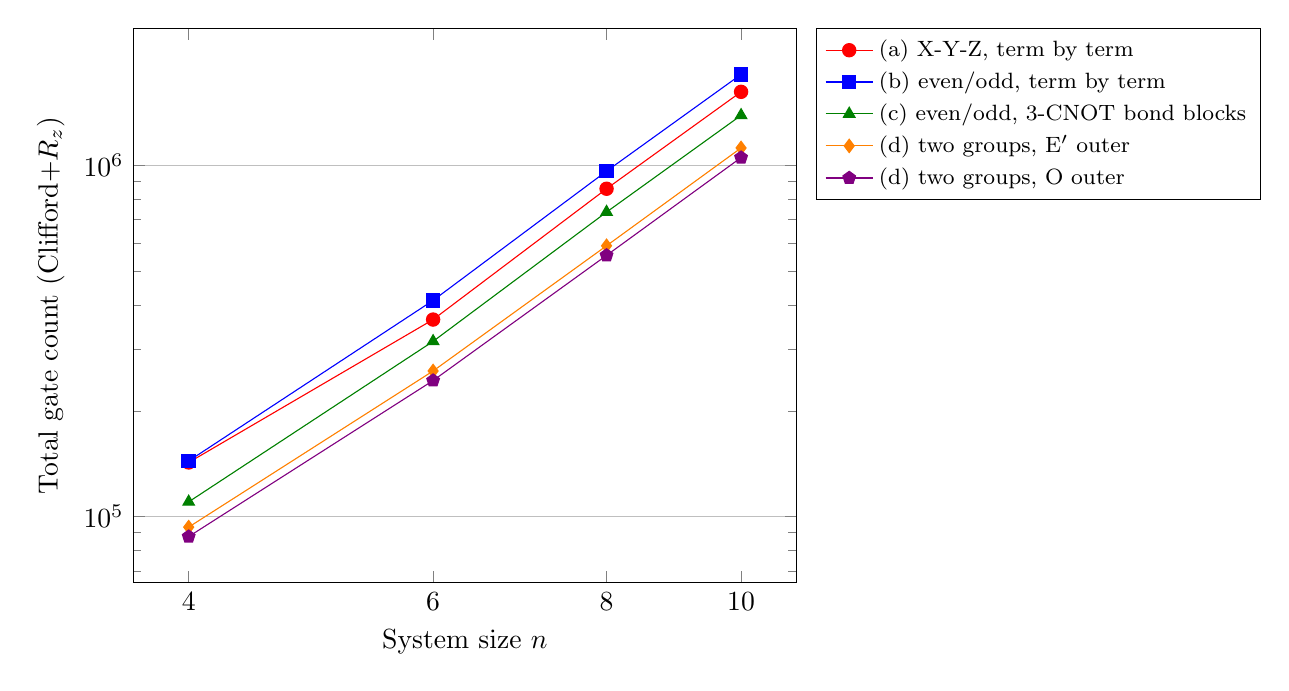
\begin{tikzpicture}
  \begin{loglogaxis}[
    width=10cm,
    xlabel={System size $n$},
    ylabel={Total gate count (Clifford+$R_z$)},
    xtick={4,6,8,10},
    xticklabels={4,6,8,10},
    ymajorgrids=true,
    legend pos=outer north east,
    legend cell align=left,
    legend style={font=\footnotesize},
  ]
    \addplot[red, mark=*, mark size=2.4pt, mark options={solid, fill=red}] coordinates {
      (4,142596)
      (6,363834)
      (8,857616)
      (10,1618740)
    };
    \addlegendentry{(a) X-Y-Z, term by term}
    \addplot[blue, mark=square*, mark size=2.4pt, mark options={solid, fill=blue}] coordinates {
      (4,144024)
      (6,412488)
      (8,962472)
      (10,1814580)
    };
    \addlegendentry{(b) even/odd, term by term}
    \addplot[green!50!black, mark=triangle*, mark size=2.4pt, mark options={solid, fill=green!50!black}] coordinates {
      (4,110136)
      (6,315432)
      (8,736008)
      (10,1387620)
    };
    \addlegendentry{(c) even/odd, 3-CNOT bond blocks}
    \addplot[orange, mark=diamond*, mark size=2.4pt, mark options={solid, fill=orange}] coordinates {
      (4,93340)
      (6,259740)
      (8,590200)
      (10,1120600)
    };
    \addlegendentry{(d) two groups, E$'$ outer}
    \addplot[violet, mark=pentagon*, mark size=2.4pt, mark options={solid, fill=violet}] coordinates {
      (4,87718)
      (6,243939)
      (8,554124)
      (10,1051945)
    };
    \addlegendentry{(d) two groups, O outer}
  \end{loglogaxis}
\end{tikzpicture}

\clearpage

\section*{\texttt{cnot-S4-by-grouping.tex}}
Suzuki $S_4$: cnot count by grouping (unmerged, measured $r$)\par\medskip
% Generated by plsimcount.pfgrouping -- do not edit; regenerate instead.
% Suzuki S4, cnot, unmerged, cz, seed 1, t = n, measured r
% git_commit=04cd66abb614bdc66fb48e891cef085a299e0ab1 git_dirty=False
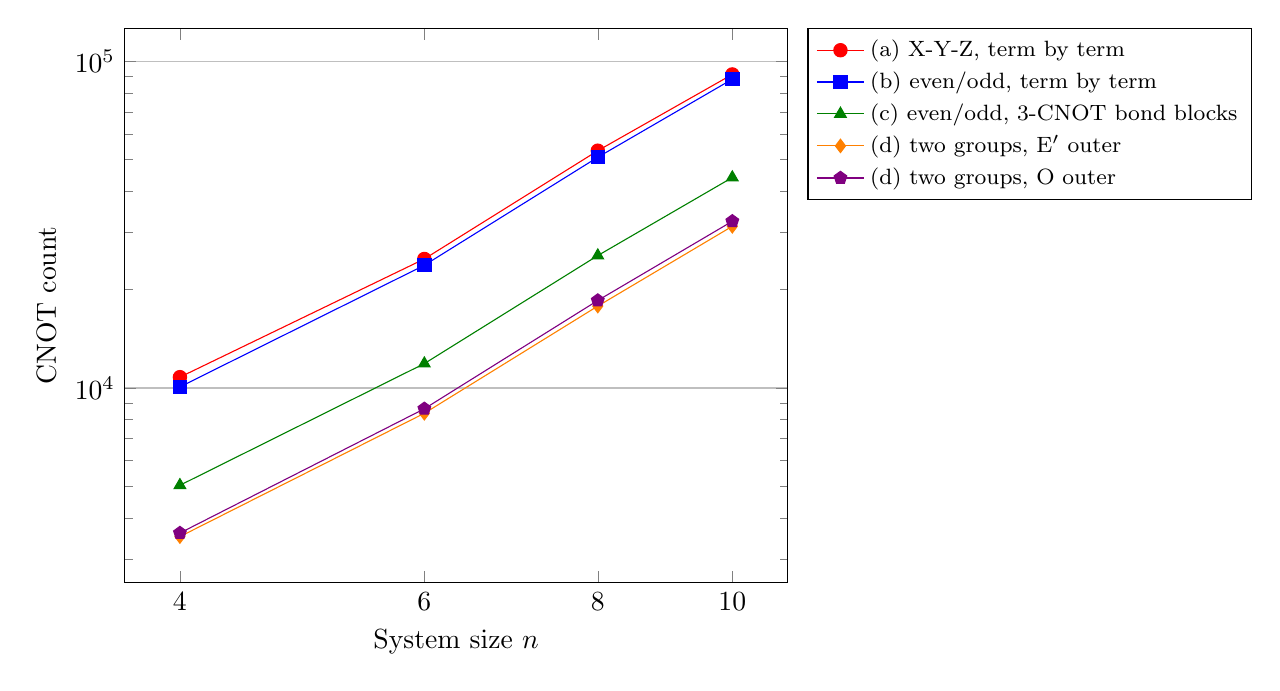
\begin{tikzpicture}
  \begin{loglogaxis}[
    width=10cm,
    xlabel={System size $n$},
    ylabel={CNOT count},
    xtick={4,6,8,10},
    xticklabels={4,6,8,10},
    ymajorgrids=true,
    legend pos=outer north east,
    legend cell align=left,
    legend style={font=\footnotesize},
  ]
    \addplot[red, mark=*, mark size=2.4pt, mark options={solid, fill=red}] coordinates {
      (4,10800)
      (6,24840)
      (8,53280)
      (10,91200)
    };
    \addlegendentry{(a) X-Y-Z, term by term}
    \addplot[blue, mark=square*, mark size=2.4pt, mark options={solid, fill=blue}] coordinates {
      (4,10080)
      (6,23760)
      (8,50880)
      (10,88200)
    };
    \addlegendentry{(b) even/odd, term by term}
    \addplot[green!50!black, mark=triangle*, mark size=2.4pt, mark options={solid, fill=green!50!black}] coordinates {
      (4,5040)
      (6,11880)
      (8,25440)
      (10,44100)
    };
    \addlegendentry{(c) even/odd, 3-CNOT bond blocks}
    \addplot[orange, mark=diamond*, mark size=2.4pt, mark options={solid, fill=orange}] coordinates {
      (4,3510)
      (6,8370)
      (8,17820)
      (10,31275)
    };
    \addlegendentry{(d) two groups, E$'$ outer}
    \addplot[violet, mark=pentagon*, mark size=2.4pt, mark options={solid, fill=violet}] coordinates {
      (4,3600)
      (6,8640)
      (8,18540)
      (10,32400)
    };
    \addlegendentry{(d) two groups, O outer}
  \end{loglogaxis}
\end{tikzpicture}

\clearpage

\section*{\texttt{total-S4-by-grouping.tex}}
Suzuki $S_4$: total count by grouping (unmerged, measured $r$)\par\medskip
% Generated by pysimcount.pfgrouping -- do not edit; regenerate instead.
% Suzuki S4, total, unmerged, cz, seed 1, t = n, measured r
% git_commit=04cd66abb614bdc66fb48e891cef085a299e0ab1 git_dirty=False
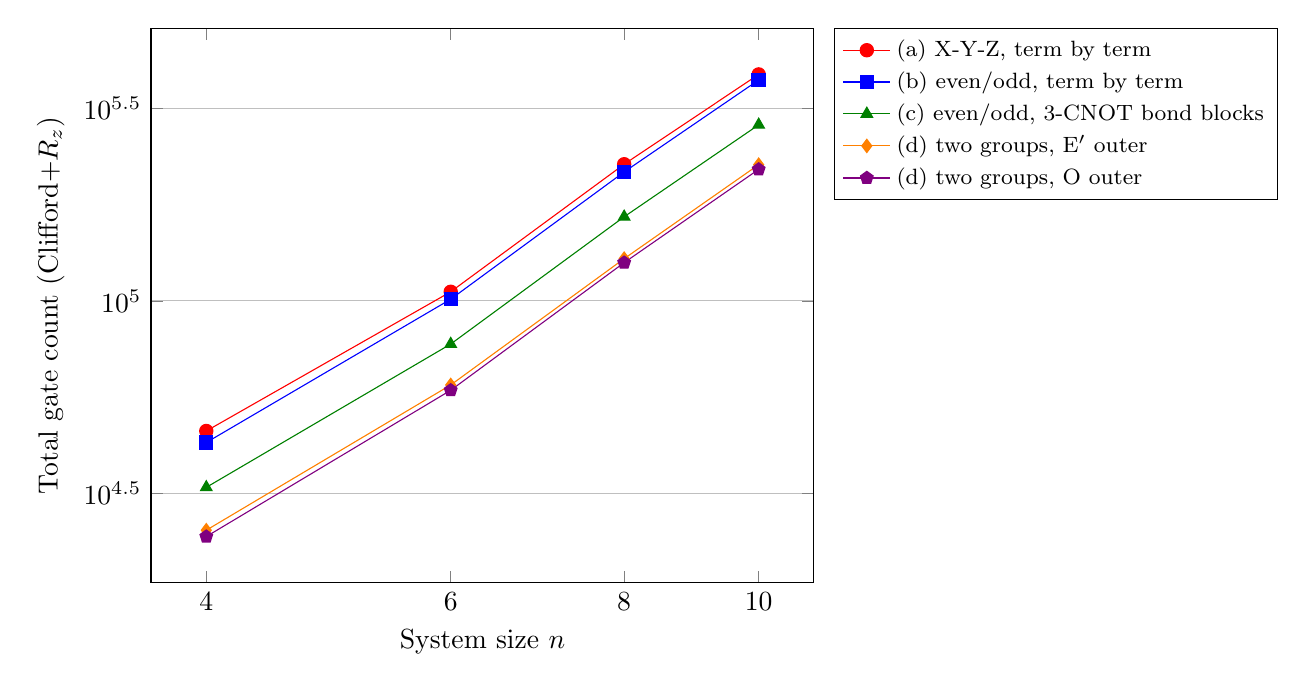
\begin{tikzpicture}
  \begin{loglogaxis}[
    width=10cm,
    xlabel={System size $n$},
    ylabel={Total gate count (Clifford+$R_z$)},
    xtick={4,6,8,10},
    xticklabels={4,6,8,10},
    ymajorgrids=true,
    legend pos=outer north east,
    legend cell align=left,
    legend style={font=\footnotesize},
  ]
    \addplot[red, mark=*, mark size=2.4pt, mark options={solid, fill=red}] coordinates {
      (4,45900)
      (6,105570)
      (8,226440)
      (10,387600)
    };
    \addlegendentry{(a) X-Y-Z, term by term}
    \addplot[blue, mark=square*, mark size=2.4pt, mark options={solid, fill=blue}] coordinates {
      (4,42840)
      (6,100980)
      (8,216240)
      (10,374850)
    };
    \addlegendentry{(b) even/odd, term by term}
    \addplot[green!50!black, mark=triangle*, mark size=2.4pt, mark options={solid, fill=green!50!black}] coordinates {
      (4,32760)
      (6,77220)
      (8,165360)
      (10,286650)
    };
    \addlegendentry{(c) even/odd, 3-CNOT bond blocks}
    \addplot[orange, mark=diamond*, mark size=2.4pt, mark options={solid, fill=orange}] coordinates {
      (4,25350)
      (6,60450)
      (8,128700)
      (10,225875)
    };
    \addlegendentry{(d) two groups, E$'$ outer}
    \addplot[violet, mark=pentagon*, mark size=2.4pt, mark options={solid, fill=violet}] coordinates {
      (4,24400)
      (6,58560)
      (8,125660)
      (10,219600)
    };
    \addlegendentry{(d) two groups, O outer}
  \end{loglogaxis}
\end{tikzpicture}

\clearpage
\end{document}
